\section{Estudos e aplicações}
\label{sec:applications}

Por último, com PR-OWL já definido formalmente e obtida uma ferramenta para construir ontologias probabilísticas foram desenvolvidos alguns estudos em situações do mundo real como o modelamento de uma ontologia marítima~\cite{Laskey11} e outra para o reconhecimento de fraudes em Brasil~\cite{Rommel13}.

\subsection{Probabilistic Ontology and Knowledge Fusion for Procurement Fraud Detection in Brazil}
\label{subsec:fraud}

Para lidar com as demandas dos cidadãos de transparência e prevenção de corrupção, a Controladoria-Geral da União organizou campanhas para educar a gente nesses temas e fiz inspeções a múltiplas instituições. Mas apesar de ter toda essa informação coletada de vários lugares (municipalidades, a Polícia Federal, etc), não tinham uma forma eficiente de unir todas elas. Além disso, a deteção de fraudes é feito manualmente por um auditor e o número de casos que pode analizar durante um tempo é limitado. O principal problema que eles tinham era a incerteza em muitos dos termos de todas as instituições. Este trabalho explica o proceso da construção de uma ontologia probabilística usando PR-OWL 2.0 para detectar fraudes em aquisições em Brasil de forma automática.

\subsection{PR-OWL 2 Case Study: A Maritime Domain Probabilistic Ontology}
\label{subsec:maritime}

Este trabalho mostra o processo necessário para mudar uma ontologia comum a uma ontologia probabilística usando como exemplo um domínio marítimo (Figura~\ref{fig:maritime}) para responder os seguintes queries:
\begin{itemize}
	\item O navio tem um terrorista?
	\item O navio tem uma rota não comum?
	\item O navio parece ter uma atitude evasiva a ataques?
	\item Qual é o tipo de aquele navio?
	\item Que bandeira pode ter aquele navio?
\end{itemize}

\begin{figure}[h]
	\centering
	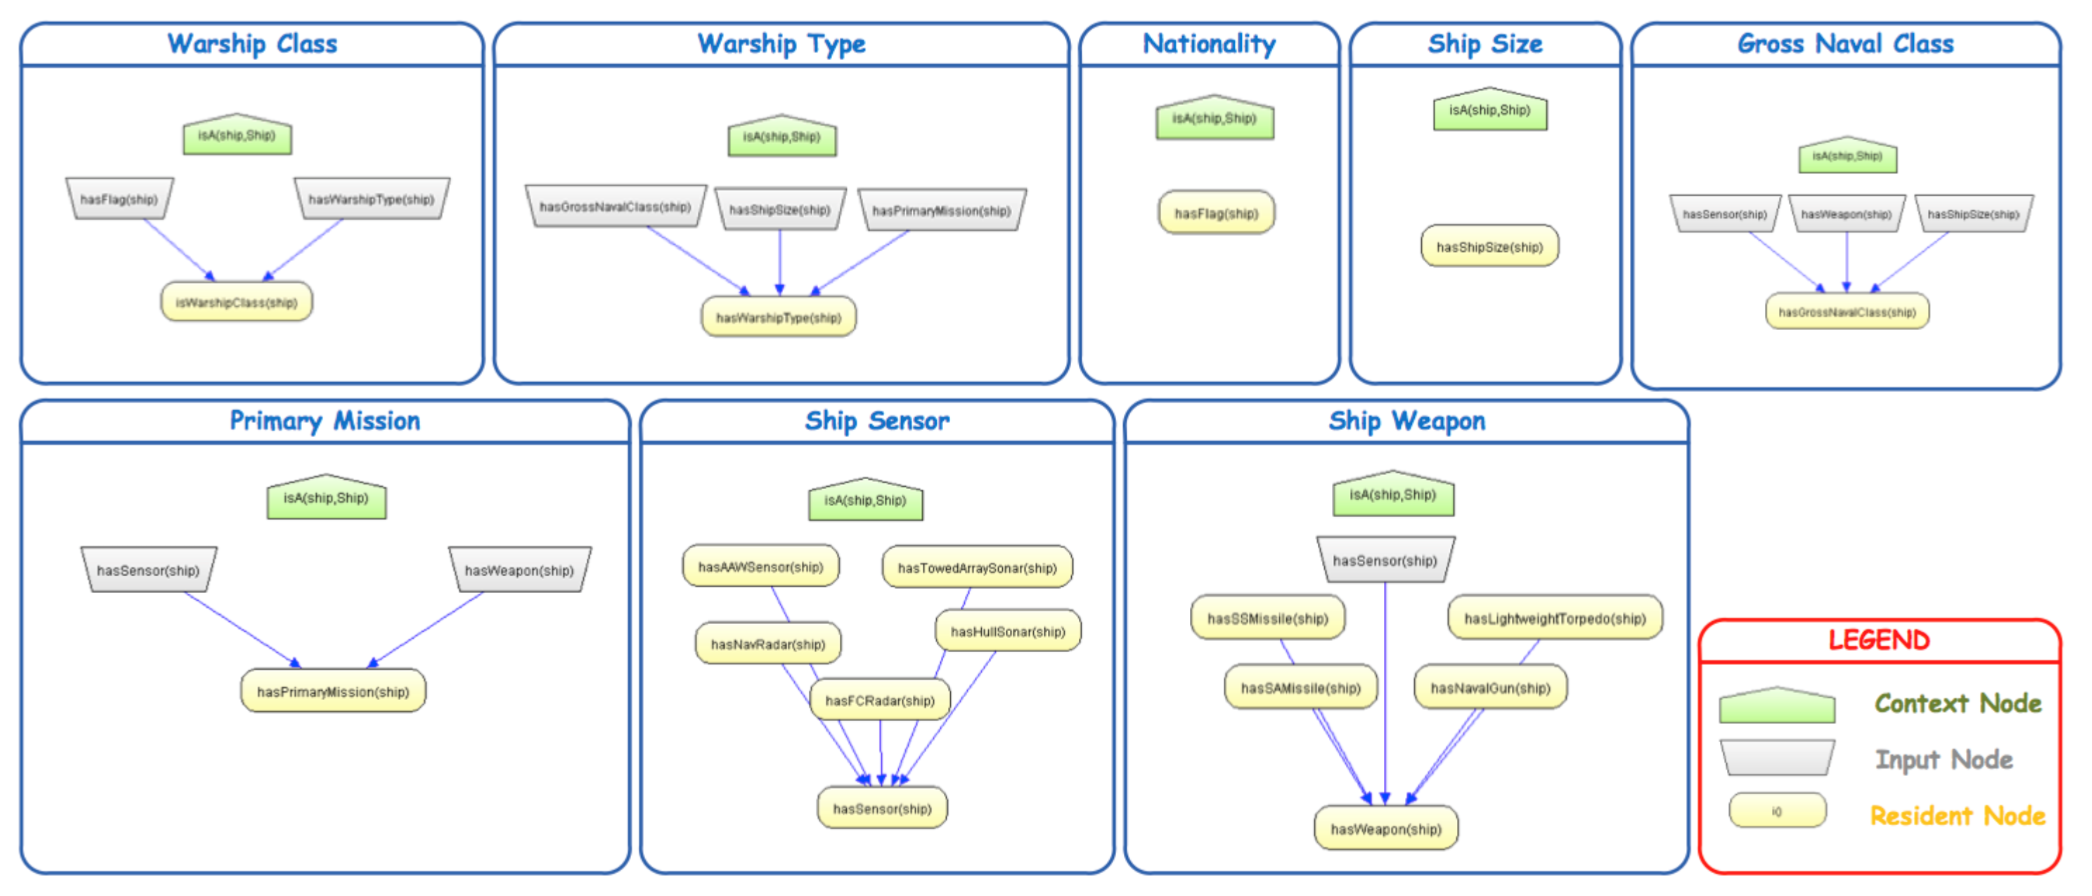
\includegraphics[height=5cm]{./images/maritime}
	\caption{Ontologia Probabilística de domínio marítimo}
	\label{fig:maritime}
\end{figure}